\documentclass[../kl10.tex]{subfiles}
\graphicspath{{\subfix{../images/}}}

\begin{document}
\section{Ein organischer Streifzug}
\textit{Hinweis: Eine Übersicht mit Abkürzungen relevanter organischer Reste findest du am Ende dieser Aufgabe.} \vspace{0.1cm}\\
Ein großes und wichtiges Teilgebiet der Chemie ist die Organische Chemie. Dabei gibt es viele grundlegende Reaktionen. Eine davon ist die Addition von Wasserstoffhalogeniden (\ce{HX}) an Doppelbindungen. Dabei wird zuerst das Proton übertragen und ein Kation gebildet. Das stabilste der möglichen Kationen führt zum Hauptprodukt. In \autoref{fig:OCSchema1}  sind vier Reaktionen gegeben, bei denen eine Addition abläuft.
\begin{figure}[H]
    \centering
    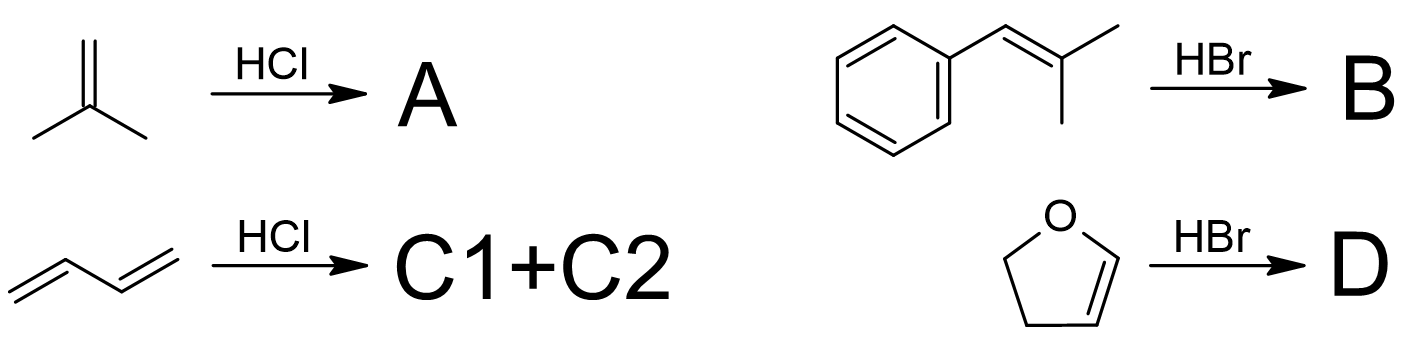
\includegraphics[width=0.85\textwidth]{2024/Abbildungen/Organik/Organik24_1.png}
    \caption{Additionen für Teilaufgabe a)}
    \label{fig:OCSchema1}
\end{figure}
\enumersteaufgabe{
\operator{Zeichne} für alle gegebenen Reaktionen die Hauptprodukte \textbf{A} bis \textbf{D}. \\Hinweis: Es entstehen \textbf{C1} und \textbf{C2} gemeinsam als Hauptprodukte.
}
\begin{tabularx}{\textwidth}{|X|X|}\hline
     \textbf{A} \solutiontext{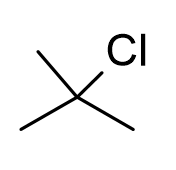
\includegraphics[width=0.2\textwidth]{2024/Abbildungen/Organik/Organik24_A.png}
     }{\vspace{4cm}} & \textbf{B}      \solutiontext{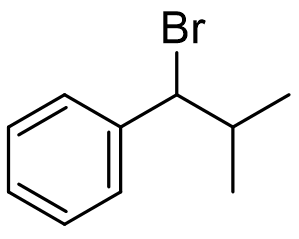
\includegraphics[width=0.22\textwidth]{2024/Abbildungen/Organik/Organik24_B.png}}{\vspace{4cm}}\\\hline
     \textbf{C1 + C2} \solutiontext{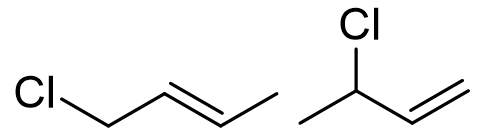
\includegraphics[width=0.35\textwidth]{2024/Abbildungen/Organik/Organik24_C.png}
     }{\vspace{4cm}} & \textbf{D}      \solutiontext{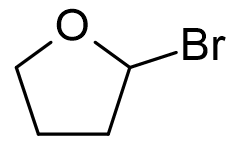
\includegraphics[width=0.26\textwidth]{2024/Abbildungen/Organik/Organik24_D.png}}{\vspace{4cm}}\\\hline
\end{tabularx}
\solutiontext{1 P. pro korrekter Strukturformel)\\
Insg. 5 P.}{}
\vspace{10pt}\\
Die Umkehrung zur Addition ist die Eliminierung. Bei dieser werden Doppelbindungen hergestellt. Wenn man zum Edukt eine Base gibt, kann diese ein Proton abspalten und die Abgangsgruppe am benachbarten Atom wird gleichzeitig abgespalten. In diesem Fall spricht man von einem E2-Mechanismus. Dabei kann die Wahl der Base Einfluss auf das Hauptprodukt nehmen, das gebildet wird. Sterisch stärker gehinderte Basen müssen Protonen angreifen, welche sterisch weniger gehindert sind. In \autoref{fig:OCSchema2} sind zwei Reaktionen dargestellt.
\begin{figure}[H]
    \centering
    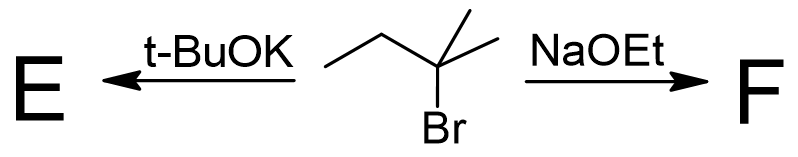
\includegraphics[width=0.5\textwidth]{2024/Abbildungen/Organik/Organik24_2.png}
    \caption{Eliminierungen mit unterschiedlichen Basen für Teilaufgabe b)}
    \label{fig:OCSchema2}
\end{figure}
\newpage
\enumaufgabe{\operator{Zeichne} das jeweilige Hauptprodukt \textbf{E} und \textbf{F} der gegebenen Reaktion.}
\begin{tabularx}{\textwidth}{|X|X|}\hline
     \textbf{E} \solutiontext{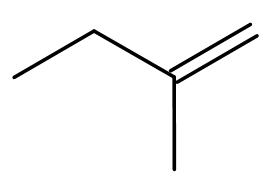
\includegraphics[width=0.3\textwidth]{2024/Abbildungen/Organik/Organik24_E.png}
     }{\vspace{6cm}} & \textbf{F}      \solutiontext{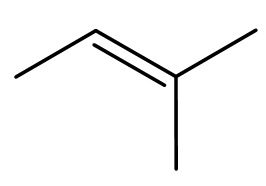
\includegraphics[width=0.3\textwidth]{2024/Abbildungen/Organik/Organik24_F.png}}{\vspace{6cm}}\\\hline
\end{tabularx}
\solutiontext{1 P. pro richtiger Strukturformel\\
Insg. 2 P.}{}
\vspace{10pt}\\
Bei Eliminierungen, die nach dem E2-Mechanismus verlaufen, können Stereozentren im Edukt die Konfiguration des Produktes eindeutig bestimmen.
\enumaufgabe{\operator{Kreuze an}, wie eine solche Reaktion genannt wird.}
\renewcommand{\arraystretch}{1.5}
\begin{tabularx}{\textwidth}{|C{0.2226\textwidth}|C{0.2226\textwidth}|C{0.2226\textwidth}|C{0.2226\textwidth}|}
    \hline
    stereobestimmend&stereoselektiv&stereospezifisch&stereotop
    \\\hline
   \emptybox&\emptybox&\solutiontext{\checkedbox}{\emptybox}&\emptybox\\\hline
\end{tabularx}
\solutiontext{0,5 P. für richtiges Kreuz; 0 P. für mehr als ein Kreuz\\
Insg. 0,5 P.}{}
\vspace{10pt}\\
In \autoref{fig:OCSchema3} werden zwei Diastereomere gezeigt, welche in einer Eliminierungsreaktion unterschiedliche Produkte ergeben.
\begin{figure}[H]
    \centering
    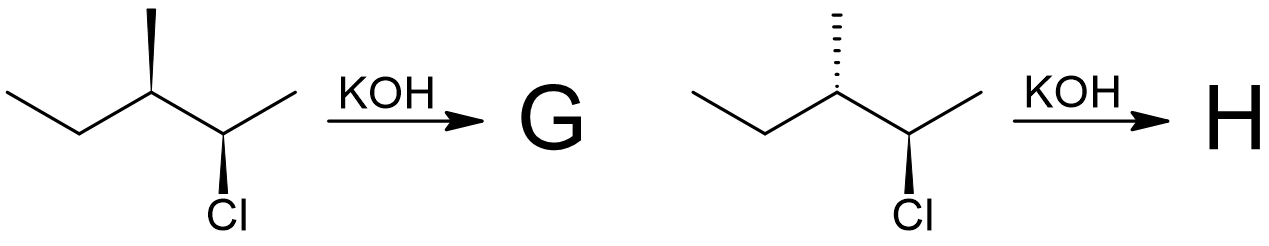
\includegraphics[width=0.7\textwidth]{2024/Abbildungen/Organik/Organik24_3.png}
    \caption{Eliminierungen für Teilaufgabe e)}
    \label{fig:OCSchema3}
\end{figure}
\enumaufgabe{\operator{Bestimme} die Konfiguration aller stereogenen Zentren nach der (R)/(S)-Nomenklatur, indem du jeweils den Stereodeskriptor an das stereogene Zentrum schreibst.}
\solution{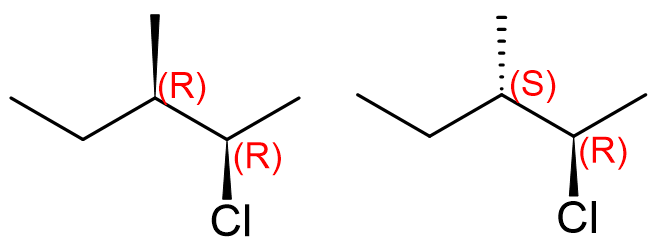
\includegraphics[width=0.3\textwidth]{2024/Abbildungen/Organik/Organik24_Stereo.png}\\
0,5 P. pro richtigem Deskriptor (Deskripor am Stereozentrum mit Chlor wird nur einmal gewertet); -0,5 Punkte für unterschiedliche Deskriptoren an Zentrum mit Chlor\\
Insg. 1,5 P.}{4cm}
\newpage
\enumaufgabe{\operator{Zeichne} die Produkte \textbf{G} und \textbf{H} unter Berücksichtigung der Stereochemie.}
\begin{tabularx}{\textwidth}{|X|X|}\hline
     \textbf{G} \solutiontext{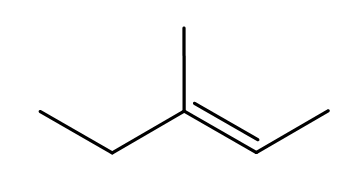
\includegraphics[width=0.3\textwidth]{2024/Abbildungen/Organik/Organik24_G.png}
     }{\vspace{6cm}} & \textbf{H}      \solutiontext{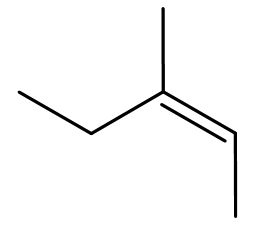
\includegraphics[width=0.23\textwidth]{2024/Abbildungen/Organik/Organik24_H.png}}{\vspace{6cm}}\\\hline
\end{tabularx}
\solutiontext{1 P. pro richtiger Strukturformel\\
Insg. 2 P.}{}
\vspace{10pt}\\
Bei allen bisher behandelten Eliminierungen entstanden immer Nebenprodukte, da die Base mehrere Protonen abspalten konnte. Mit einer besonderen Reaktion, die auf der Chemie des Siliciums basiert, kann dieses Problem umgangen werden. Die \textsc{Peterson}-Eliminierung basiert auf der hohen Affinität von Silicium zu stark elektronegativen Elementen wie Fluor oder Sauerstoff. In \autoref{fig:OCSchema4} ist ein Schritt der Synthese der Antikrebsverbindung Taxol gezeigt, bei der so ausschließlich das thermodynamisch instabilere Alken erhalten wird.
\begin{figure}[H]
    \centering
    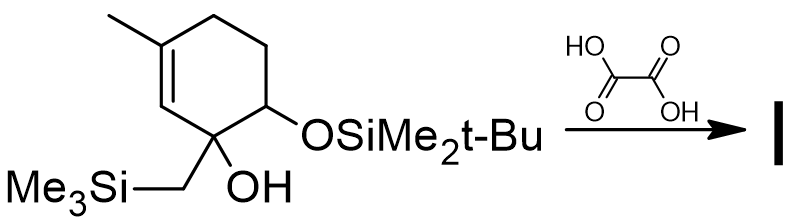
\includegraphics[width=0.6\textwidth]{2024/Abbildungen/Organik/Organik24_4.png}
    \caption{Syntheseschritt aus der Synthese von Taxol für Teilaufgabe f)}
    \label{fig:OCSchema4}
\end{figure}
\enumaufgabe{\operator{Zeichne} die Verbindung \textbf{I}. \\Hinweis: Das Siliciumatom am Sauerstoffatom nimmt nicht an der Reaktion teil, sondern ist eine Schutzgruppe.}
\solution{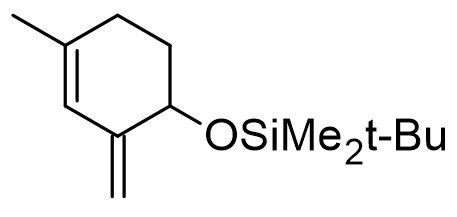
\includegraphics[width=0.5\textwidth]{2024/Abbildungen/Organik/Organik24_I.png}\\
2 P. für korrekte Strukturformel; 0 P. für Veresterung mit Oxalsäure; 0 P. für Alkene im Ring\\
Insg. 2 P.}{6cm}
\newpage

Eine konkurrierende Reaktion zur Eliminierung ist die nucleophile Substitution.



\enumaufgabe{\operator{Zeichne} die Mechanismen der miteinander konkurrierenden $\mathrm{E2}$- und $\mathrm{S_N2}$-Reaktionen an Chlorethan mit einem Hydroxid-Ion.}
\solution{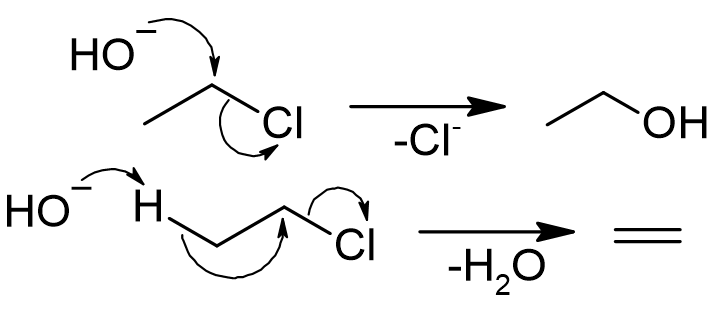
\includegraphics[width=0.5\textwidth]{2024/Abbildungen/Organik/Organik24_Mechanismen.png}\\
0,5 P. für korrekte Edukte (bei beiden Reaktionen); 0,5 P. für korrektes organisches Produkt ($\mathrm{S_N2}$); 0,5 P. für korrektes organisches Produkt (E2); 0,5 P. für korrekte Elektronenflusspfeile; -0,5 P. falls min. einmal Nebenprodukte fehlen oder falsch sind\\
Insg. 2 P.}{6cm}
Erneut nimmt der Mechanismus der $\mathrm{S_N2}$-Reaktion gegenüber dem der $\mathrm{S_N1}$-Reaktion einen besonderen Stellenwert ein, weil man auch hier die Stereochemie direkt durch das Edukt kontrollieren kann.
\enumaufgabe{\operator{Begründe} kurz, warum bei einer $\mathrm{S_N1}$-Reaktion die Stereochemie des Edukts nicht die Stereochemie des Produkts bestimmt. \\\operator{Benenne} die Mischnung der Isomere.}
\solution{\noindent Bei einer $\mathrm{S_N1}$-Reaktion bildet sich ein planares Carbokation (0,5 P.). Bei diesem ist der Angriff von beiden Seiten gleich wahrscheinlich (0,5 P.). Das Produktgemisch wird Racemat genannt (0,5 P.).\\
Insg. 1,5 P.}{2cm}
Diese Art der Reaktion kann auch in der organischen Synthese angewendet werden. In \autoref{fig:OCSchema5} ist ein Synthesevorschlag abgebildet, wie das Epoxid \textbf{L} hergestellt werden kann. Dabei wird zuerst ein Enolat erzeugt und dieses wird in situ (wird direkt im Reaktionsgefäß weiterverwendet) mit Brom umgesetzt.
\begin{figure}[H]
    \centering
    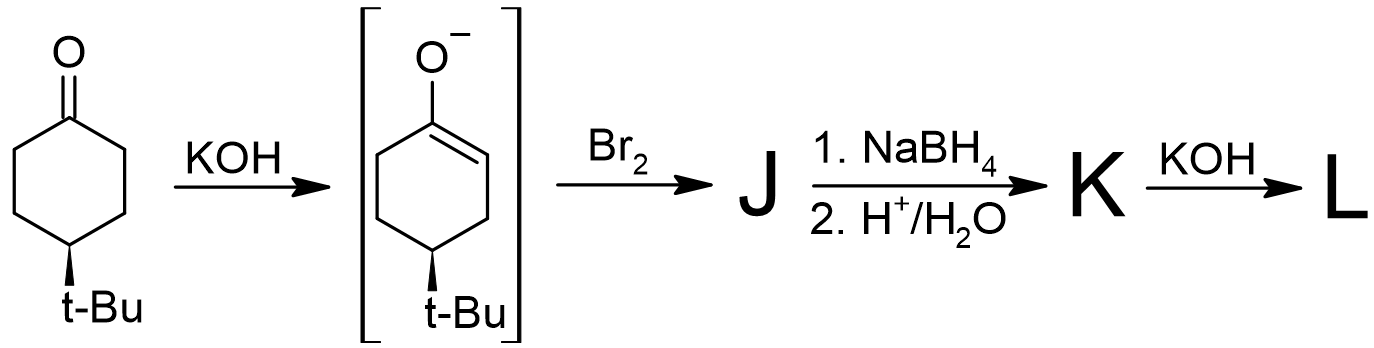
\includegraphics[width=0.9\textwidth]{2024/Abbildungen/Organik/Organik24_5.png}
    \caption{Syntheseschema für i)}
    \label{fig:OCSchema5}
\end{figure}
\textbf{Hinweise:}
\begin{itemize}
    \item \textbf{J} besitzt genau ein Bromatom.
    \item \ce{NaBH4} ist ein Hydriddonator.
    \item \ce{H^+/H2O} ist die wässrige Aufarbeitung des Zwischenproduktes, das bei dieser Reaktion entsteht.
    \item Bei einem Epoxid ist ein Sauerstoffatom an zwei benachbarte Kohlenstoffatome gebunden.
    \item Die Bildung des Epoxids \textbf{L} geschieht durch eine intramolekulare $\mathrm{S_N2}$-Reaktion.
\end{itemize}
\newpage
\enumaufgabe{\operator{Zeichne} alle möglichen Stereoisomere für die Produkte \textbf{J} bis \textbf{L}. \\\operator{Umkreise} ein Zwischenprodukt, wenn es den nächsten Schritt im Schema nicht eingehen kann. }
\begin{tabularx}{\textwidth}{|X|X|}\hline
     \textbf{J} \solutiontext{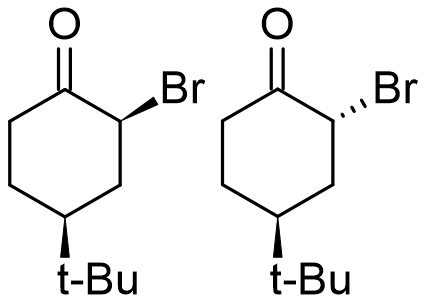
\includegraphics[width=0.3\textwidth]{2024/Abbildungen/Organik/Organik24_J.png}
     }{\vspace{8cm}} & \textbf{K}      \solutiontext{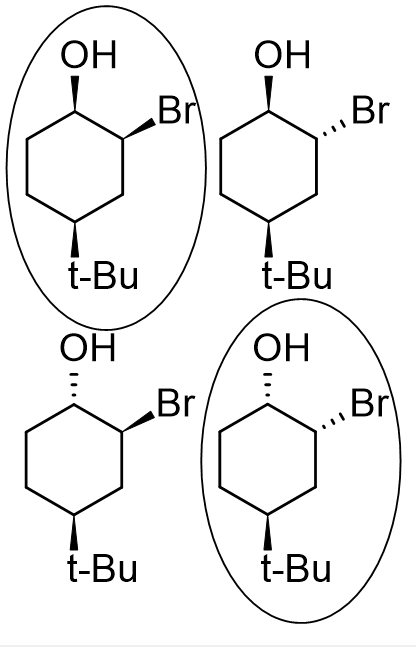
\includegraphics[width=0.3\textwidth]{2024/Abbildungen/Organik/Organik24_K.png}}{\vspace{8cm}}\\\hline
     \textbf{L} \solutiontext{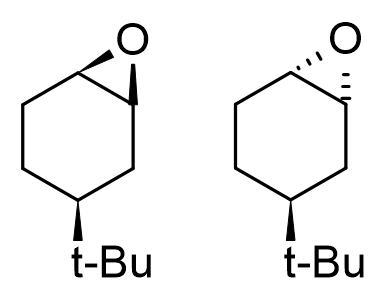
\includegraphics[width=0.3\textwidth]{2024/Abbildungen/Organik/Organik24_L.png}
     }{\vspace{8cm}} &\\\hline
\end{tabularx}
\solutiontext{1 P. pro richtiger Strukturformel; -1 P. falls eine Strukturformel doppelt; 0,5 P. für jedes korrekt umkreiste Produkt; -0,5 P. für jedes falsch umkreiste Produkt\\
Insg. 9 P.}{}
\vspace{10pt}\\
\textbf{Übersicht über Abkürzungen relevanter organischer Reste:}
\begin{figure}[H]
    \centering
    \includegraphics[width=0.5\textwidth]{2024/Abbildungen/Organik/Organik24_Abkürzungen.png}
\end{figure}
\vspace{0,5cm}
\solutiontext{$\sum$ 25,5 P.}{}
\end{document}